\documentclass[supercite]{Experimental_Report}

\title{~~~~~~数据结构实验~~~~~~}
\author{赵大进}
%\coauthor{张三、李四}
\school{计算机科学与技术学院}
\classnum{CS2110}
\stunum{U202115630}
%\costunum{U202115631、U202115631}
\instructor{陈加忠} % 该系列实验报告模板有华科大计院教师陈加忠制作
\date{2021年11月11日}

\usepackage{algorithm, multirow}
\usepackage{algpseudocode}
\usepackage{amsmath}
\usepackage{amsthm}
\usepackage{framed}
\usepackage{mathtools}
\usepackage{subcaption}
\usepackage{xltxtra} %提供了针对XeTeX的改进并且加入了XeTeX的LOGO, 自动调用xunicode宏包(提供Unicode字符宏)
\usepackage{bm}
\usepackage{tikz}
\usepackage{tikzscale}
\usepackage{pgfplots}
%\usepackage{enumerate}

\pgfplotsset{compat=1.16}

\newcommand{\cfig}[3]{
  \begin{figure}[htb]
    \centering
    \includegraphics[width=#2\textwidth]{images/#1.tikz}
    \caption{#3}
    \label{fig:#1}
  \end{figure}
}

\newcommand{\sfig}[3]{
  \begin{subfigure}[b]{#2\textwidth}
    \includegraphics[width=\textwidth]{images/#1.tikz}
    \caption{#3}
    \label{fig:#1}
  \end{subfigure}
}

\newcommand{\xfig}[3]{
  \begin{figure}[htb]
    \centering
    #3
    \caption{#2}
    \label{fig:#1}
  \end{figure}
}

\newcommand{\rfig}[1]{\autoref{fig:#1}}
\newcommand{\ralg}[1]{\autoref{alg:#1}}
\newcommand{\rthm}[1]{\autoref{thm:#1}}
\newcommand{\rlem}[1]{\autoref{lem:#1}}
\newcommand{\reqn}[1]{\autoref{eqn:#1}}
\newcommand{\rtbl}[1]{\autoref{tbl:#1}}

\algnewcommand\Null{\textsc{null }}
\algnewcommand\algorithmicinput{\textbf{Input:}}
\algnewcommand\Input{\item[\algorithmicinput]}
\algnewcommand\algorithmicoutput{\textbf{Output:}}
\algnewcommand\Output{\item[\algorithmicoutput]}
\algnewcommand\algorithmicbreak{\textbf{break}}
\algnewcommand\Break{\algorithmicbreak}
\algnewcommand\algorithmiccontinue{\textbf{continue}}
\algnewcommand\Continue{\algorithmiccontinue}
\algnewcommand{\LeftCom}[1]{\State $\triangleright$ #1}

\newtheorem{thm}{定理}[section]
\newtheorem{lem}{引理}[section]

\colorlet{shadecolor}{black!15}

\theoremstyle{definition}
\newtheorem{alg}{算法}[section]

\def\thmautorefname~#1\null{定理~#1~\null}
\def\lemautorefname~#1\null{引理~#1~\null}
\def\algautorefname~#1\null{算法~#1~\null}

\begin{document}

\maketitle

\clearpage

\pagenumbering{Roman}

\tableofcontents[level=2]

\clearpage

\pagenumbering{arabic}

\section{基于顺序存储结构的线性表实现}

图\ref{fig1-1}只是网页整体框架举例,它是用visio画的,然后再在visio里通过文件-打印,如图\ref{fig1-2}所示打印成pdf文件,然后再用pdf阅览器的工具,如图\ref{fig1-3}所示,做适当的裁剪。画图说明网页的整体框架,进行简要的文字描述等。画图说明网页的整体框架,进行简要的文字描述等。画图说明网页的整体框架,进行简要的文字描述等。画图说明网页的整体框架,进行简要的文字描述等。画图说明网页的整体框架,进行简要的文字描述等。画图说明网页的整体框架,进行简要的文字描述等。画图说明网页的整体框架,进行简要的文字描述等。

请注意,当正文中出现1) 2) 3)罗列时,请必须用enumerate环境,具体如下!

\begin{enumerate}
\renewcommand{\labelenumi}{\theenumi)}
	\item C++
	\item Java
	\item HTML
\end{enumerate}

画图说明网页的整体框架,进行简要的文字描述等。画图说明网页的整体框架,进行简要的文字描述等。画图说明网页的整体框架,进行简要的文字描述等。画图说明网页的整体框架,进行简要的文字描述等。画图说明网页的整体框架,进行简要的文字描述等。画图说明网页的整体框架,进行简要的文字描述等。画图说明网页的整体框架,进行简要的文字描述等。

\subsection{问题描述}

说明此实验要解决的基本问题。大力出奇迹!!!参考文献无法显示怎么办?陈老师正在想办法解决\cite{STR2021Neurocom, AVS2021Neurocom}!我是参考文献。我是第二小节\cite{Mehrabian1974An}。我是第二小节\cite{Rezaei2014CVPR}。我是第二小节\cite{Ramnath2008IJCV}。

\subsection{系统设计}

包括整体系统结构设计和数据结构设计等。先在文件夹里的bib文件里添加新的参考文献,给每篇参考文献取一个索引的名字,然后再引用比如\cite{STR2021Neurocom}\cite{AVS2021Neurocom, Rezaei2014CVPR}。请注意书籍、期刊论文、专利等bib条目的格式是不一样的。画图说明网页的整体框架,进行简要的文字描述等。画图说明网页的整体框架,进行简要的文字描述等。画图说明网页的整体框架,进行简要的文字描述等。画图说明网页的整体框架,进行简要的文字描述等。画图说明网页的整体框架,进行简要的文字描述等。画图说明网页的整体框架,进行简要的文字描述等。画图说明网页的整体框架,进行简要的文字描述等。

\subsection{系统实现}

主要说明各个主要函数的实现思想,复杂函数可辅助流程图进行说明,函数和系统实现的源代码放在附录中。画图说明网页的整体框架,进行简要的文字描述等。画图说明网页的整体框架,进行简要的文字描述等。画图说明网页的整体框架,进行简要的文字描述等。画图说明网页的整体框架,进行简要的文字描述等。画图说明网页的整体框架,进行简要的文字描述等。画图说明网页的整体框架,进行简要的文字描述等。画图说明网页的整体框架,进行简要的文字描述等。

\subsection{系统测试}

主要说明针对各个函数正常和异常的测试用例及测试结果画图说明网页的整体框架,进行简要的文字描述等。画图说明网页的整体框架,进行简要的文字描述等。画图说明网页的整体框架,进行简要的文字描述等。画图说明网页的整体框架,进行简要的文字描述等。画图说明网页的整体框架,进行简要的文字描述等。画图说明网页的整体框架,进行简要的文字描述等。画图说明网页的整体框架,进行简要的文字描述等。

\begin{figure}[htb] % here top bottom
	\begin{center}
		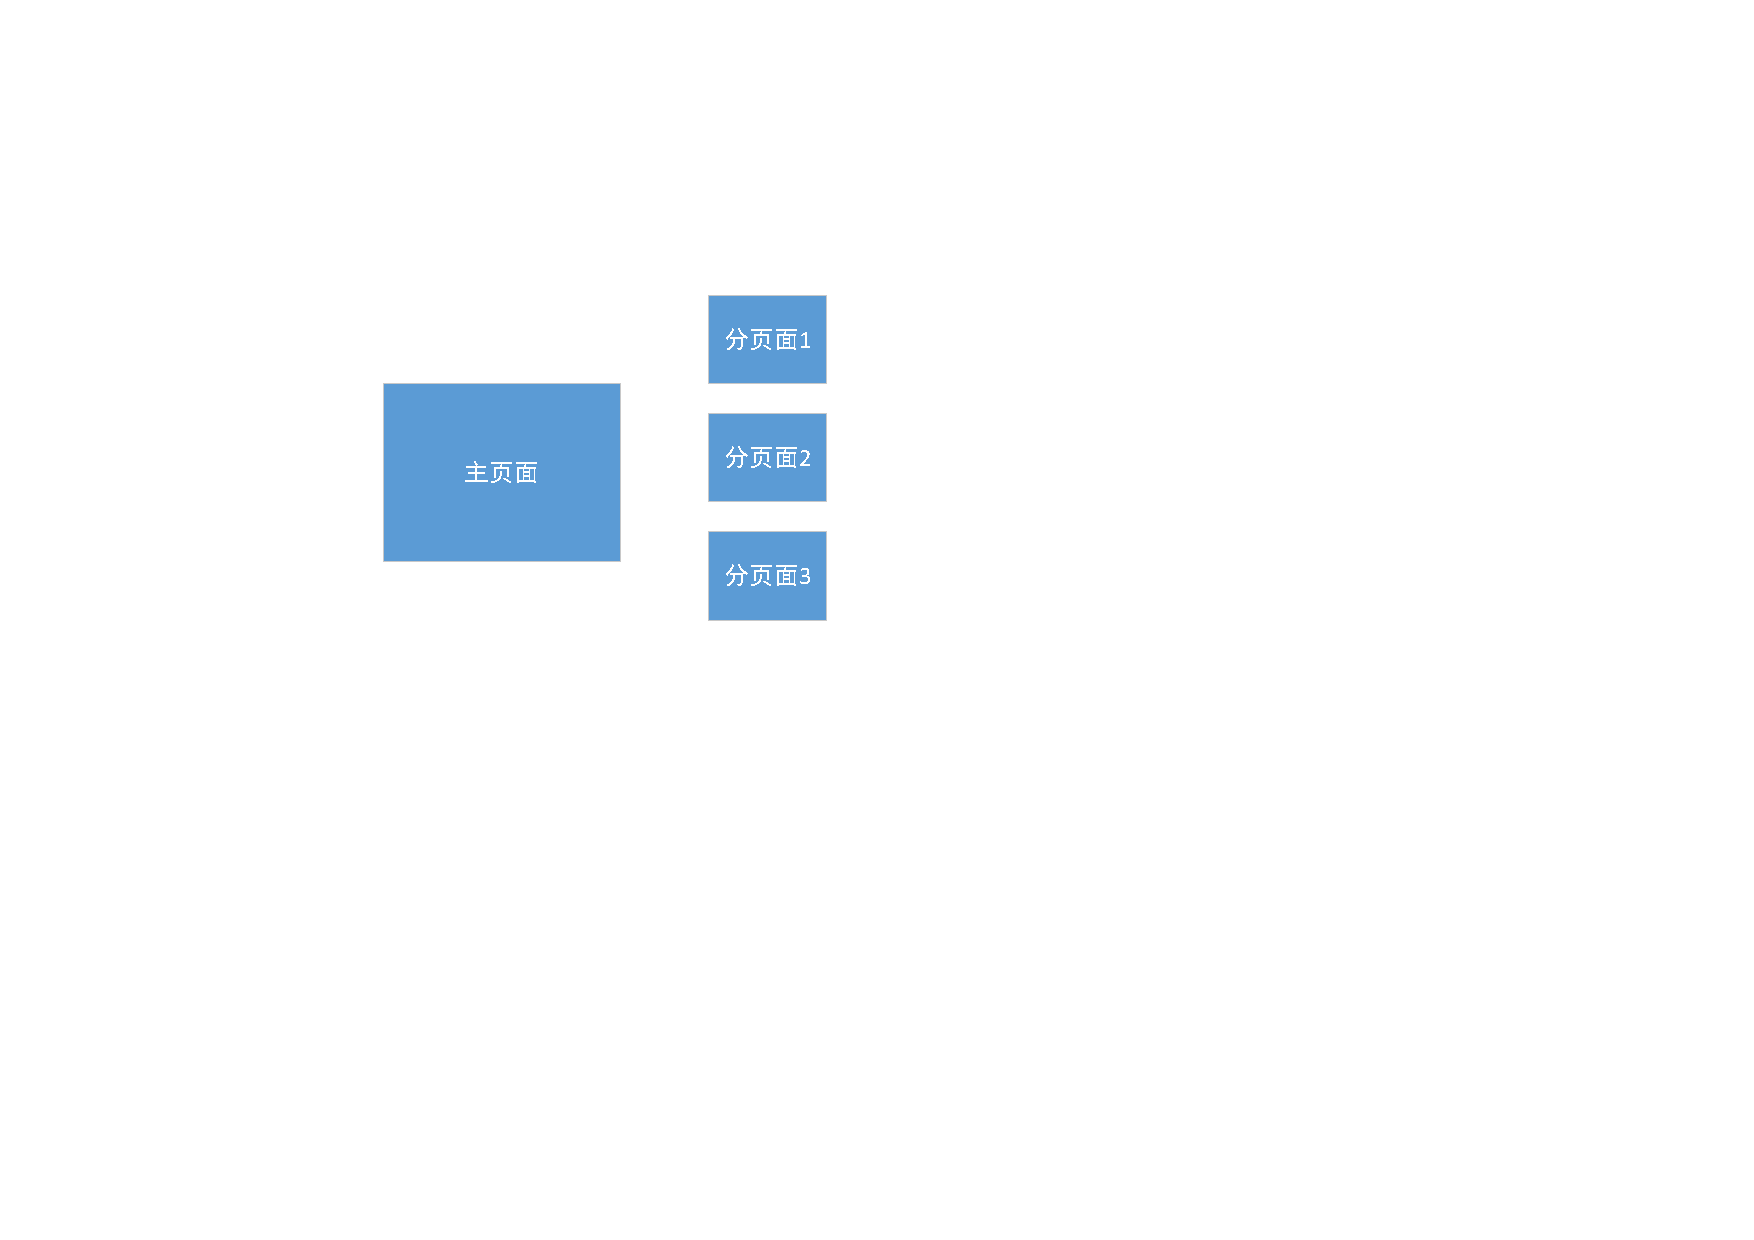
\includegraphics[scale=0.80]{images/1-1.pdf}
		\caption{网页整体框架举例}
		\label{fig1-1}
	\end{center}
\end{figure}

\subsection{实验小结}

重点说明在实验中取得的实际经验,例如调试中碰到的典型错误等,不要写套话。画图说明网页的整体框架,进行简要的文字描述等。画图说明网页的整体框架,进行简要的文字描述等。画图说明网页的整体框架,进行简要的文字描述等。画图说明网页的整体框架,进行简要的文字描述等。画图说明网页的整体框架,进行简要的文字描述等。画图说明网页的整体框架,进行简要的文字描述等。画图说明网页的整体框架,进行简要的文字描述等。

\begin{figure}[htb]
	\begin{center}
		
\includegraphics[scale=0.60]{images/1-2.png}
		\caption{在visio里通过文件-打印,把visio图打印成pdf文件}
		\label{fig1-2}
	\end{center}
\end{figure}

画图说明网页的整体框架,进行简要的文字描述等。画图说明网页的整体框架,进行简要的文字描述等。画图说明网页的整体框架,进行简要的文字描述等。画图说明网页的整体框架,进行简要的文字描述等。画图说明网页的整体框架,进行简要的文字描述等。画图说明网页的整体框架,进行简要的文字描述等。画图说明网页的整体框架,进行简要的文字描述等。

\begin{figure}[htb]
	\begin{center}
		
\includegraphics[scale=0.50]{images/1-3.png}
		\caption{用pdf阅览器的工具,对打印得到pdf图做适当的裁剪}
		\label{fig1-3}
	\end{center}
\end{figure}

其实吧,用Latex写公式也不是很难,请参照公式\ref{equ_loss}。画表格就更简单了,请看表\ref{table2}。

\begin{eqnarray}\label{equ_loss}
	\mathcal{L}_{id}=\sum_{j=1}^{c}1\{l_k=j\}\log\frac{\exp(f_j(\textbf{W},x_k))}{\sum\nolimits_{l=1}^{c}\exp(f_l(\textbf{W},x_k))}
\end{eqnarray}

画图说明网页的整体框架,进行简要的文字描述等。画图说明网页的整体框架,进行简要的文字描述等。画图说明网页的整体框架,进行简要的文字描述等。画图说明网页的整体框架,进行简要的文字描述等。画图说明网页的整体框架,进行简要的文字描述等。画图说明网页的整体框架,进行简要的文字描述等。画图说明网页的整体框架,进行简要的文字描述等。

\begin{table}
	\begin{center}
		\setlength{\tabcolsep}{2.0mm}
		\caption{Mean and standard deviation of estimation error (Euler angles) on Pandora. The best performance is in \textbf{bold}.}
		\label{table2}
		\begin{tabular}{c|ccccc}
			\hline
			Method    			        & Data               & Pitch         & Roll           & Yaw              & Accuracy\\
			\hline
			\hline			
			\multirow{5}{*}{POSEidon}   & Depth              & 6.5 $\pm$ 6.6  & 5.4 $\pm$ 5.1  & 10.4 $\pm$ 11.8  & 0.646\\
			& FfD              	 & 6.8 $\pm$ 7.0  & 5.7 $\pm$ 5.7  & 10.5 $\pm$ 14.6  & 0.647\\
			& Gray-level         & 7.1 $\pm$ 6.6  & 5.6 $\pm$ 5.8  & 9.0  $\pm$ 10.9  & 0.639\\
			& Depth + FfD	     & 5.6 $\pm$ 5.0  & 4.9 $\pm$ 5.0  & 9.8  $\pm$ 13.4  & 0.698\\
			& Depth + FfD + MI   & 5.7 $\pm$ 5.6  & 4.9 $\pm$ 5.1  & 9.0  $\pm$ 11.9  & 0.715\\
			\hline
			DRF                         & Depth              & 6.2 $\pm$ 9.5  & 4.6 $\pm$ 6.7  & 9.3  $\pm$ 14.6  & --\\
			\hline
			\multirow{3}{*}{Ours}   	& Depth              & 5.9 $\pm$ 6.2  & 4.5 $\pm$ 4.9  & 8.8  $\pm$ 10.9  & 0.666\\
			& RGB                & 5.5 $\pm$ 5.3  & 4.4 $\pm$ 5.5  & 8.6  $\pm$ 9.3   & 0.698\\
			& RGB + Depth        & 5.0 $\pm$ 4.8  & 4.3 $\pm$ 4.9  & 8.1  $\pm$ 8.3   & \textbf{0.737}\\
			\hline
		\end{tabular}
	\end{center}
\end{table}

\newpage

\section{基于链式存储结构的线性表实现}

描述主页的结构,给出主页截图,描述主要设计思路等,请见图\ref{fig2-1}。描述主页的结构,给出主页截图,描述主要设计思路等。描述主页的结构,给出主页截图,描述主要设计思路等。描述主页的结构,给出主页截图,描述主要设计思路等。描述主页的结构,给出主页截图,描述主要设计思路等。描述主页的结构,给出主页截图,描述主要设计思路等。描述主页的结构,给出主页截图,描述主要设计思路等。

\begin{figure}[htb]
	\begin{center}
		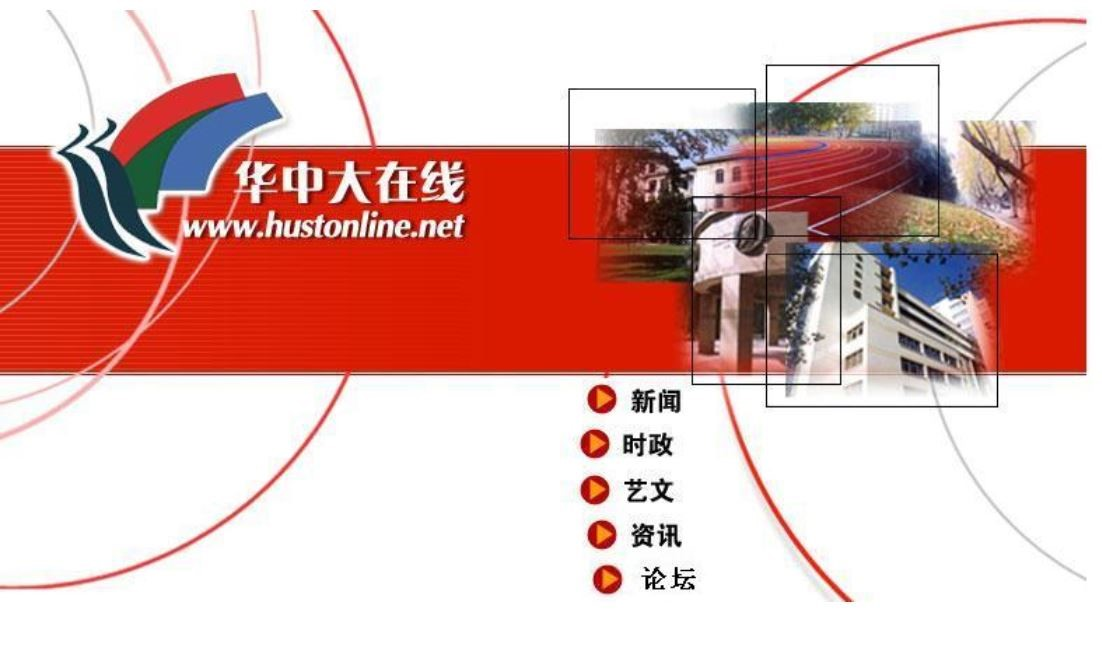
\includegraphics[scale=0.40]{images/2-1.jpg}
		\caption{主页举例}
		\label{fig2-1}
	\end{center}
\end{figure}

\subsection{问题描述}

说明此实验要解决的基本问题。大力出奇迹!!!参考文献无法显示怎么办?陈老师正在想办法解决\cite{STR2021Neurocom, AVS2021Neurocom}!我是参考文献。我是第二小节\cite{Mehrabian1974An}。我是第二小节\cite{Rezaei2014CVPR}。我是第二小节\cite{Ramnath2008IJCV}。

\subsection{系统设计}

包括整体系统结构设计和数据结构设计等。先在文件夹里的bib文件里添加新的参考文献,给每篇参考文献取一个索引的名字,然后再引用比如\cite{STR2021Neurocom}\cite{AVS2021Neurocom, Rezaei2014CVPR}。请注意书籍、期刊论文、专利等bib条目的格式是不一样的。画图说明网页的整体框架,进行简要的文字描述等。画图说明网页的整体框架,进行简要的文字描述等。画图说明网页的整体框架,进行简要的文字描述等。画图说明网页的整体框架,进行简要的文字描述等。画图说明网页的整体框架,进行简要的文字描述等。画图说明网页的整体框架,进行简要的文字描述等。画图说明网页的整体框架,进行简要的文字描述等。

\subsection{系统实现}

主要说明各个主要函数的实现思想,复杂函数可辅助流程图进行说明,函数和系统实现的源代码放在附录中。画图说明网页的整体框架,进行简要的文字描述等。画图说明网页的整体框架,进行简要的文字描述等。画图说明网页的整体框架,进行简要的文字描述等。画图说明网页的整体框架,进行简要的文字描述等。画图说明网页的整体框架,进行简要的文字描述等。画图说明网页的整体框架,进行简要的文字描述等。画图说明网页的整体框架,进行简要的文字描述等。

\subsection{系统测试}

主要说明针对各个函数正常和异常的测试用例及测试结果画图说明网页的整体框架,进行简要的文字描述等。画图说明网页的整体框架,进行简要的文字描述等。画图说明网页的整体框架,进行简要的文字描述等。画图说明网页的整体框架,进行简要的文字描述等。画图说明网页的整体框架,进行简要的文字描述等。画图说明网页的整体框架,进行简要的文字描述等。画图说明网页的整体框架,进行简要的文字描述等。

\begin{figure}[htb] % here top bottom
	\begin{center}
		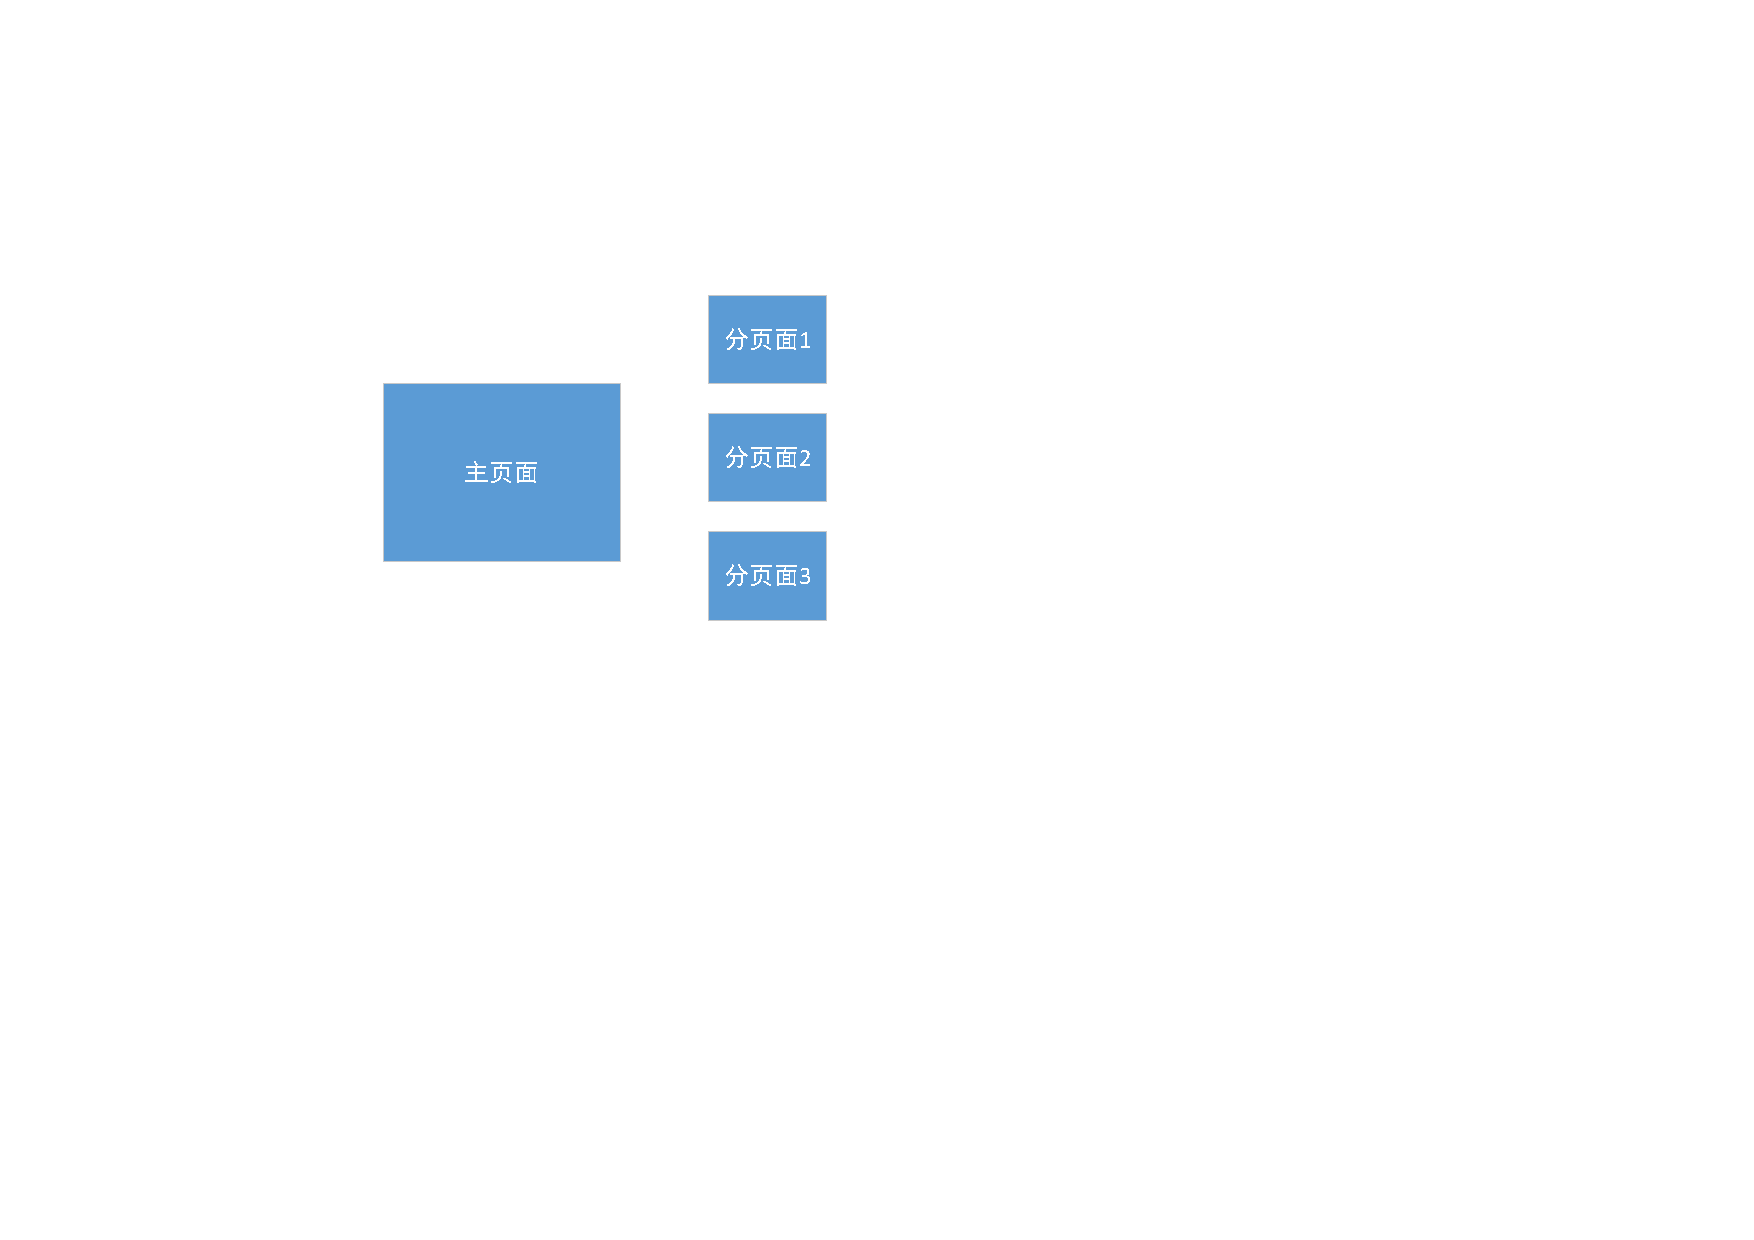
\includegraphics[scale=0.80]{images/1-1.pdf}
		\caption{网页整体框架举例}
		\label{fig4-1}
	\end{center}
\end{figure}

\subsection{实验小结}

\newpage

\section{基于二叉链表的二叉树实现}

给出分页面截图,描述主要设计思路等。给出分页面截图,描述主要设计思路等。给出分页面截图,描述主要设计思路等。给出分页面截图,描述主要设计思路等。

\subsection{问题描述}

说明此实验要解决的基本问题。大力出奇迹!!!参考文献无法显示怎么办?陈老师正在想办法解决\cite{STR2021Neurocom, AVS2021Neurocom}!我是参考文献。我是第二小节\cite{Mehrabian1974An}。我是第二小节\cite{Rezaei2014CVPR}。我是第二小节\cite{Ramnath2008IJCV}。

\subsection{系统设计}

包括整体系统结构设计和数据结构设计等。先在文件夹里的bib文件里添加新的参考文献,给每篇参考文献取一个索引的名字,然后再引用比如\cite{STR2021Neurocom}\cite{AVS2021Neurocom, Rezaei2014CVPR}。请注意书籍、期刊论文、专利等bib条目的格式是不一样的。画图说明网页的整体框架,进行简要的文字描述等。画图说明网页的整体框架,进行简要的文字描述等。画图说明网页的整体框架,进行简要的文字描述等。画图说明网页的整体框架,进行简要的文字描述等。画图说明网页的整体框架,进行简要的文字描述等。画图说明网页的整体框架,进行简要的文字描述等。画图说明网页的整体框架,进行简要的文字描述等。

\subsection{系统实现}

主要说明各个主要函数的实现思想,复杂函数可辅助流程图进行说明,函数和系统实现的源代码放在附录中。画图说明网页的整体框架,进行简要的文字描述等。画图说明网页的整体框架,进行简要的文字描述等。画图说明网页的整体框架,进行简要的文字描述等。画图说明网页的整体框架,进行简要的文字描述等。画图说明网页的整体框架,进行简要的文字描述等。画图说明网页的整体框架,进行简要的文字描述等。画图说明网页的整体框架,进行简要的文字描述等。

\subsection{系统测试}

主要说明针对各个函数正常和异常的测试用例及测试结果画图说明网页的整体框架,进行简要的文字描述等。画图说明网页的整体框架,进行简要的文字描述等。画图说明网页的整体框架,进行简要的文字描述等。画图说明网页的整体框架,进行简要的文字描述等。画图说明网页的整体框架,进行简要的文字描述等。画图说明网页的整体框架,进行简要的文字描述等。画图说明网页的整体框架,进行简要的文字描述等。

\begin{figure}[htb] % here top bottom
	\begin{center}
		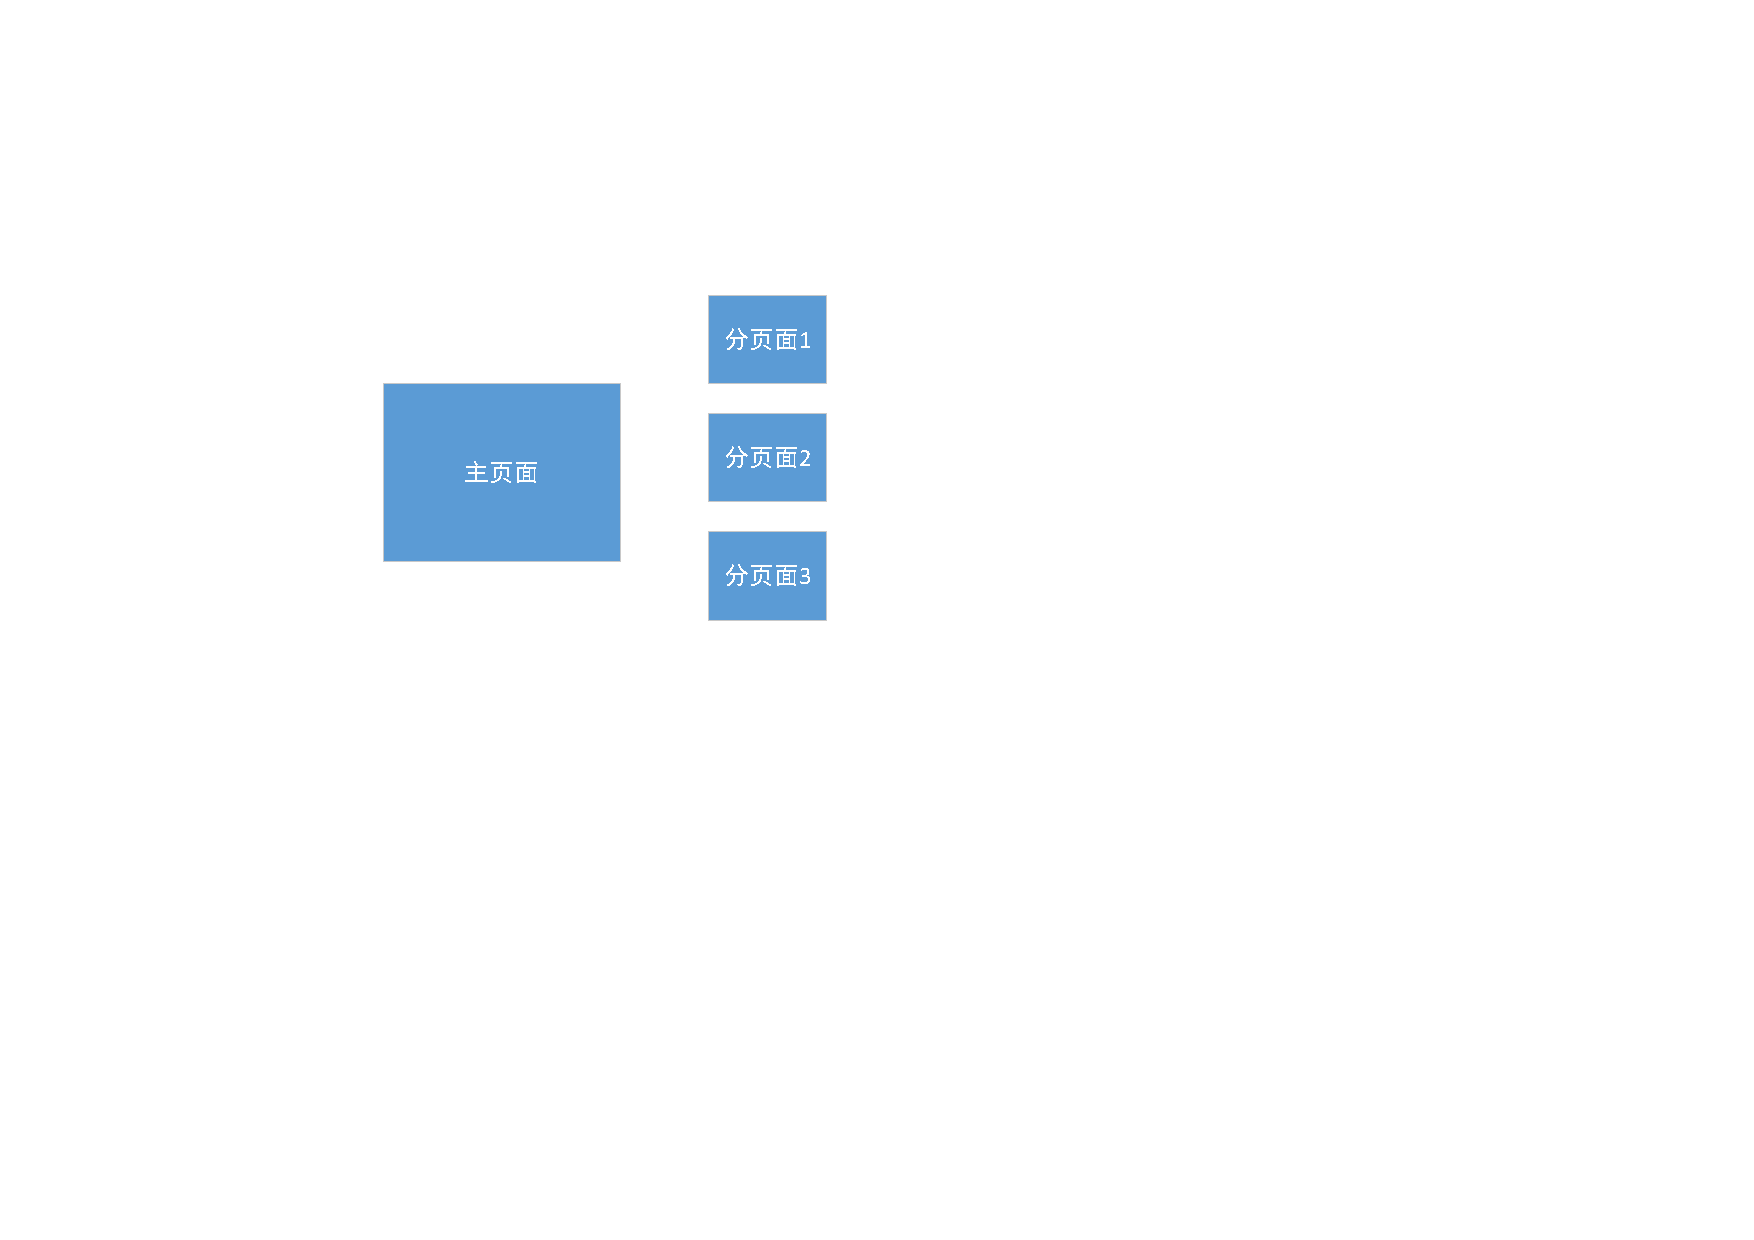
\includegraphics[scale=0.80]{images/1-1.pdf}
		\caption{网页整体框架举例}
		\label{fig3-1}
	\end{center}
\end{figure}

\subsection{实验小结}

如果实验报告中要用到算法伪代码,请参考算法\ref{alg:1},也可以参考算法\ref{alg:2}。如果实验报告中要用到算法伪代码,请参考算法\ref{alg:1},也可以参考算法\ref{alg:2}。如果实验报告中要用到算法伪代码,请参考算法\ref{alg:1},也可以参考算法\ref{alg:2}。如果实验报告中要用到算法伪代码,请参考算法\ref{alg:1},也可以参考算法\ref{alg:2}。

\begin{shaded*}\begin{alg}{一个复杂算法}
		\label{alg:1}
		\begin{algorithmic}
			\Input Two numbers $a$ and $b$
			\Output The sum of $a$ and $b$
			\Procedure{A-Plus-B}{$a, b$}
			\If $a = 0$
			\State \Return $b$
			\EndIf
			\State $res \gets 0$
			\While{$b \neq 0$}
			\State Increase $res$ by $1$
			\State $b \gets b - 1$
			\EndWhile
			\State \Return $res$
			\EndProcedure
		\end{algorithmic}
\end{alg}\end{shaded*}

如果实验报告中要用到算法伪代码,请参考算法\ref{alg:1},也可以参考算法\ref{alg:2}。如果实验报告中要用到算法伪代码,请参考算法\ref{alg:1},也可以参考算法\ref{alg:2}。如果实验报告中要用到算法伪代码,请参考算法\ref{alg:1},也可以参考算法\ref{alg:2}。如果实验报告中要用到算法伪代码,请参考算法\ref{alg:1},也可以参考算法\ref{alg:2}。

\begin{algorithm}[h] 
	\caption{一个更复杂算法}
	\begin{algorithmic}[1]
		\State Initialization: $I_{xy}$, $z_{f}=Zeros(128, 128)$; 
		\For{$0\leq n \textless N$}
		\State $i=\lfloor x_n \rfloor+64$, $j=\lfloor y_n \rfloor + 64$
		\If{$z_n<0$ and $|z_n|>|z_{f}(i,j)|$};
		\State $z_{f}(i,j)=z_n$;
		\EndIf
		\State $I_{xy}(i,j)=z_{f}(i,j)$;
		\EndFor 
	\end{algorithmic}\label{alg:2}
\end{algorithm}

\newpage

\section{基于邻接表的图实现}

\subsection{问题描述}

说明此实验要解决的基本问题。大力出奇迹!!!参考文献无法显示怎么办?陈老师正在想办法解决\cite{STR2021Neurocom, AVS2021Neurocom}!我是参考文献。我是第二小节\cite{Mehrabian1974An}。我是第二小节\cite{Rezaei2014CVPR}。我是第二小节\cite{Ramnath2008IJCV}。

\subsection{系统设计}

包括整体系统结构设计和数据结构设计等。先在文件夹里的bib文件里添加新的参考文献,给每篇参考文献取一个索引的名字,然后再引用比如\cite{STR2021Neurocom}\cite{AVS2021Neurocom, Rezaei2014CVPR}。请注意书籍、期刊论文、专利等bib条目的格式是不一样的。画图说明网页的整体框架,进行简要的文字描述等。画图说明网页的整体框架,进行简要的文字描述等。画图说明网页的整体框架,进行简要的文字描述等。画图说明网页的整体框架,进行简要的文字描述等。画图说明网页的整体框架,进行简要的文字描述等。画图说明网页的整体框架,进行简要的文字描述等。画图说明网页的整体框架,进行简要的文字描述等。

\subsection{系统实现}

主要说明各个主要函数的实现思想,复杂函数可辅助流程图进行说明,函数和系统实现的源代码放在附录中。画图说明网页的整体框架,进行简要的文字描述等。画图说明网页的整体框架,进行简要的文字描述等。画图说明网页的整体框架,进行简要的文字描述等。画图说明网页的整体框架,进行简要的文字描述等。画图说明网页的整体框架,进行简要的文字描述等。画图说明网页的整体框架,进行简要的文字描述等。画图说明网页的整体框架,进行简要的文字描述等。

\subsection{系统测试}

主要说明针对各个函数正常和异常的测试用例及测试结果画图说明网页的整体框架,进行简要的文字描述等。画图说明网页的整体框架,进行简要的文字描述等。画图说明网页的整体框架,进行简要的文字描述等。画图说明网页的整体框架,进行简要的文字描述等。画图说明网页的整体框架,进行简要的文字描述等。画图说明网页的整体框架,进行简要的文字描述等。画图说明网页的整体框架,进行简要的文字描述等。

\begin{figure}[htb] % here top bottom
	\begin{center}
		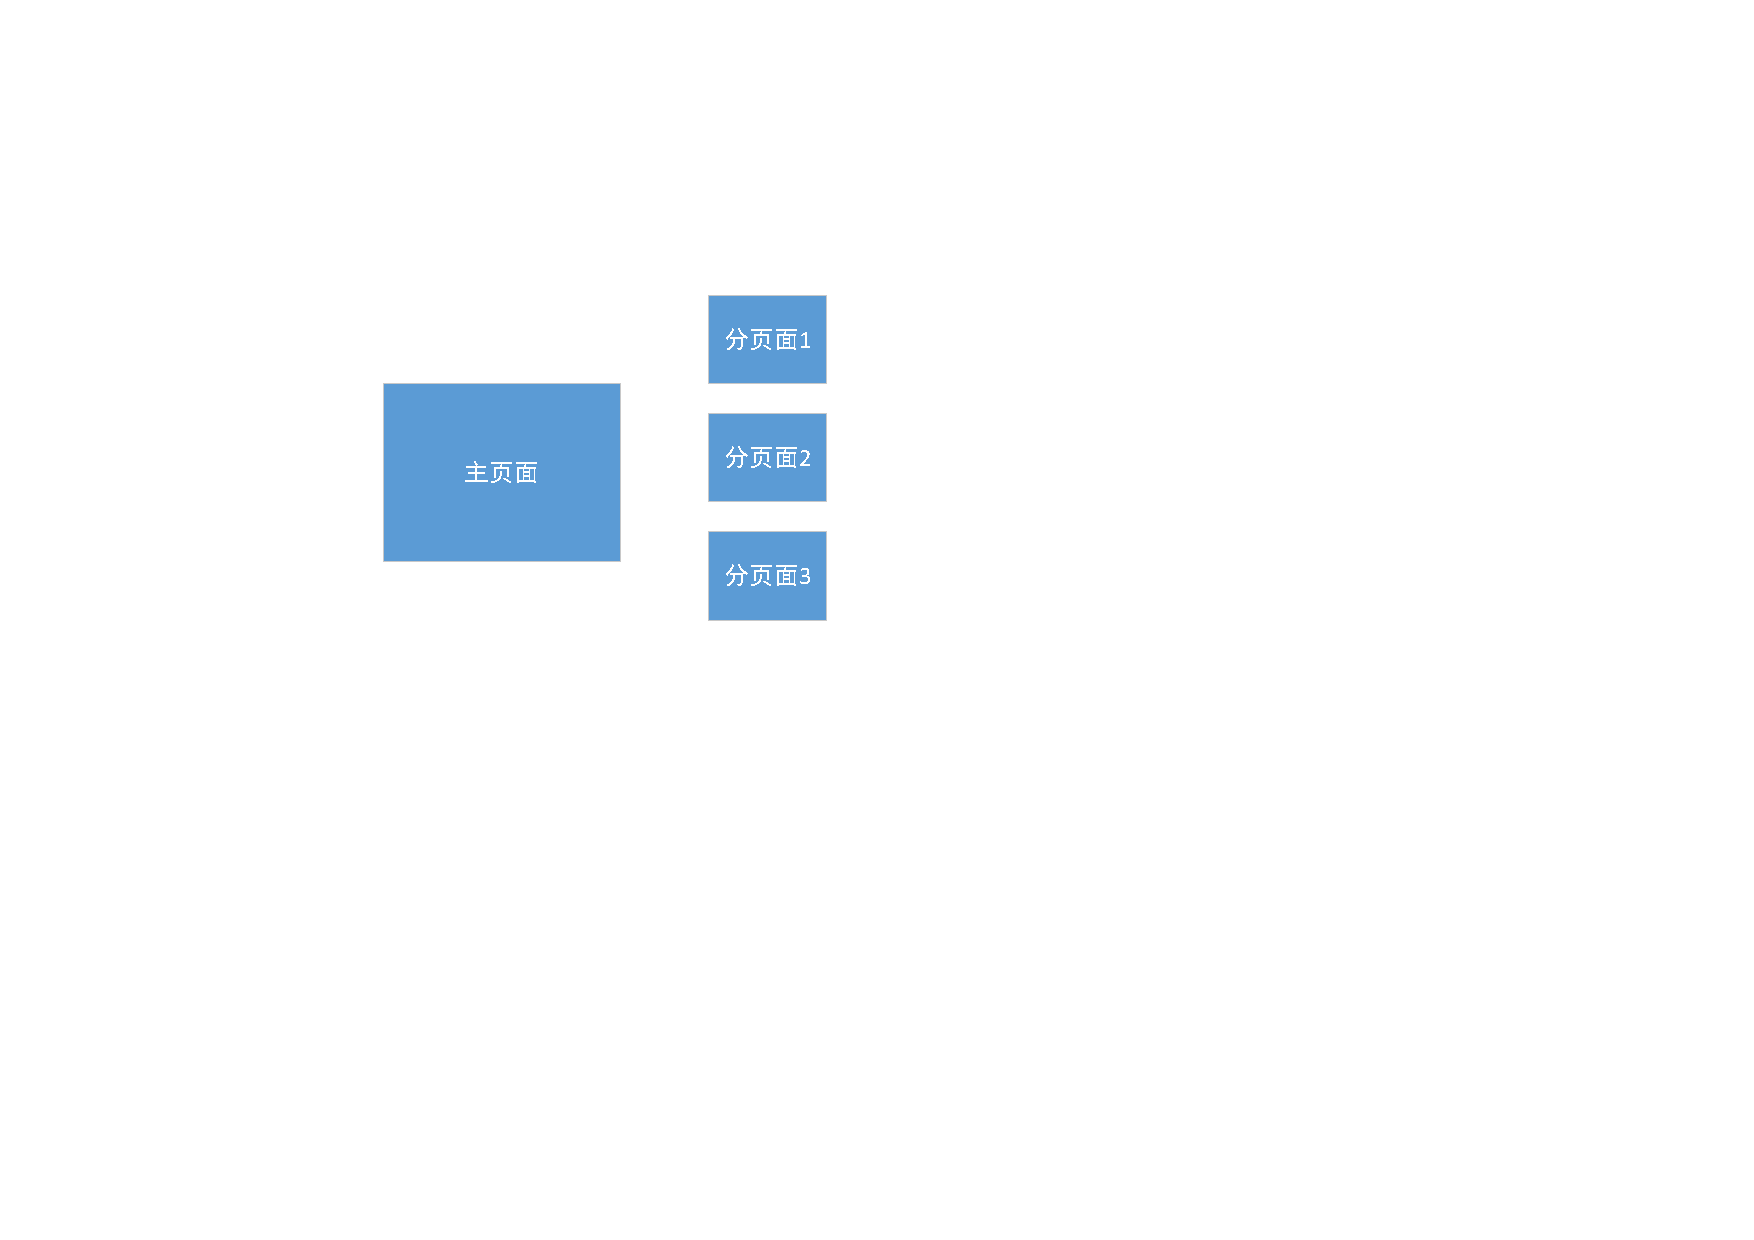
\includegraphics[scale=0.80]{images/1-1.pdf}
		\caption{网页整体框架举例}
		\label{fig5-1}
	\end{center}
\end{figure}

\subsection{实验小结}

\newpage

\section{课程的收获和建议}

描述通过学习该专题,有何收获,有何建议,如某专题可适当减少讲授时间、某专题可适当增加讲授内容和时间等。描述通过学习该专题,有何收获,有何建议,如某专题可适当减少讲授时间、某专题可适当增加讲授内容和时间等。描述通过学习该专题,有何收获,有何建议,如某专题可适当减少讲授时间、某专题可适当增加讲授内容和时间等。描述通过学习该专题,有何收获,有何建议,如某专题可适当减少讲授时间、某专题可适当增加讲授内容和时间等。

\subsection{基于顺序存储结构的线性表实现}

描述通过学习计算机基础知识专题,有何收获,有何建议,如某专题可适当减少讲授时间、某专题可适当增加讲授内容和时间等。描述网页的设计和实现过程中遇到的问题及如何解决。描述网页的设计和实现过程中遇到的问题及如何解决。描述网页的设计和实现过程中遇到的问题及如何解决。描述网页的设计和实现过程中遇到的问题及如何解决。描述网页的设计和实现过程中遇到的问题及如何解决。描述网页的设计和实现过程中遇到的问题及如何解决。描述网页的设计和实现过程中遇到的问题及如何解决。描述网页的设计和实现过程中遇到的问题及如何解决。

\subsection{基于链式存储结构的线性表实现}

描述通过学习文档撰写工具LaTeX专题,有何收获,有何建议,如某专题可适当减少讲授时间、某专题可适当增加讲授内容和时间等。描述通过学习文档撰写工具LaTeX专题,有何收获,有何建议,如某专题可适当减少讲授时间、某专题可适当增加讲授内容和时间等。

\subsection{基于二叉链表的二叉树实现}

描述通过学习编程工具Python专题,有何收获,有何建议,如某专题可适当减少讲授时间、某专题可适当增加讲授内容和时间等。描述通过学习编程工具Python专题,有何收获,有何建议,如某专题可适当减少讲授时间、某专题可适当增加讲授内容和时间等。

\subsection{基于二叉链表的二叉树实现}

描述通过学习计算机基础知识专题,有何收获,有何建议,如某专题可适当减少讲授时间、某专题可适当增加讲授内容和时间等。描述通过学习计算机基础知识专题,有何收获,有何建议,如某专题可适当减少讲授时间、某专题可适当增加讲授内容和时间等。


\nocite{*} %% 作用是不对文献进行引用,但可以生成文献列表

\bibliographystyle{Experimental_Report}
\bibliography{Experimental_Report}
\setcounter{secnumdepth}{0}
\appendix

\section{附录A 基于顺序存储结构线性表实现的源程序}

\noindent
/* Linear Table On Sequence Structure */\\
\#include <stdio.h>\\
\#include <malloc.h>\\
\#include <stdlib.h>\\

\noindent
/*---------page 10 on textbook ---------*/\\
\#define TRUE 1\\
\#define FALSE 0\\
\#define OK 1\\
\#define ERROR 0\\
\#define INFEASTABLE -1\\
\#define OVERFLOW -2\\
\newpage
\section{附录B 基于链式存储结构线性表实现的源程序}
\newpage
\section{附录C 基于二叉链表二叉树实现的源程序}
\newpage
\section{附录D 基于邻接表图实现的源程序}

\end{document}